\documentclass[11pt, a4paper]{article}
\usepackage{graphicx,wrapfig}
\usepackage[margin=2cm]{geometry}
\usepackage[acronym]{glossaries}
\usepackage[sorting=none, style=nature]{biblatex} %Imports biblatex package
\usepackage[hidelinks]{hyperref}
\usepackage{titling}
\usepackage{float}
\usepackage{caption}

\renewcommand{\familydefault}{\sfdefault}
\newcommand{\customcite}[2]{\mbox{
  {\small \copyright} \textit{#1} \cite{#2}}
}

\newcommand{\subtitle}[1]{%
  \posttitle{%
    \par\end{center}
    \begin{center}\LARGE#1\end{center}
    \vskip0.5em}%
}

\hypersetup{
  colorlinks   = true, %Colours links instead of ugly boxes
  urlcolor     = blue, %Colour for external hyperlinks
  linkcolor    = blue, %Colour of internal links
  citecolor   = red %Colour of citations
}

\addbibresource{references.bib} %Import the bibliography file

\makenoidxglossaries
\loadglsentries{glossary.tex}



\title{\textbf{ \\{\Huge Compte Rendu de Stage Master 2}}}
\subtitle{Galaxies Pop III, premières phases de la formation des métaux et poussières dans l'Univers à très grand Redshift (6 $<$ z $<$ ?)}
\author{Dewachter Tim}
\date{25 Mars 2024 - 28 Juin 2024}

\begin{document}

\maketitle

\newpage

\tableofcontents

\newpage

\section{Introduction}

%TODO

\subsection{Contexte}

En seulement 2 ans d'opérations, le \gls{jwst} nous a déjà ouvert de nombreuses portes jusqu'alors inaccessibles, et cela dans de nombreuses branches de l'astrophysique. Grâce à ses instruments spectroscopiques et sa sensibilité à l'infrarouge proche et moyen, il est désormais possible de sonder l'univers comme jamais auparavant. Parmi les nombreux objectifs que l'on souhaite accomplir avec ce télescope, l'un d'eux est l'étude de la formation des galaxies, de l'apparition des métaux au sein de celles-ci, et de la recherche des hypothétiques galaxies de Population III, constituées d'étoiles de métallicité nulle, formées par le gaz primordial d'Hydrogène et d'Hélium.

Ce nouvel horizon sur l'univers lointain nous permet de remonter l'histoire de l'univers comme jamais auparavant. \cite{2023arXiv230600953M} %TODO



\section{Méthodologie}

\subsection{JWST et NIRSpec}

Le \gls{jwst} est un télescope spatial de 6.5 mètres de diamètre équivalent, en orbite autour du point de Lagrange L2, et actif depuis juillet 2022 \cite{jwst_website}. Sa sensibilité dans l'infrarouge en fait un outil remarquable pour observer l'univers jeune. En effet, de par l'expansion de l'univers, la lumière des objets lointains se retrouve décalée vers le rouge : il s'agit du redshift $z$, défini comme 

\begin{equation}
    1 + z = \frac{\lambda_{obs}}{\lambda_{rest}}
\end{equation}

Avec $\lambda_{obs}$ la longueur d'onde observée, et $\lambda_{rest}$ la longueur d'onde dans le référentiel de la source (au repos). Ainsi, regarder loin dans l'espace est équivalent à regarder loin dans le passé et nécessite d'observer à des longueurs d'ondes de plus en plus grandes.

\begin{figure}[H]
  \centering
  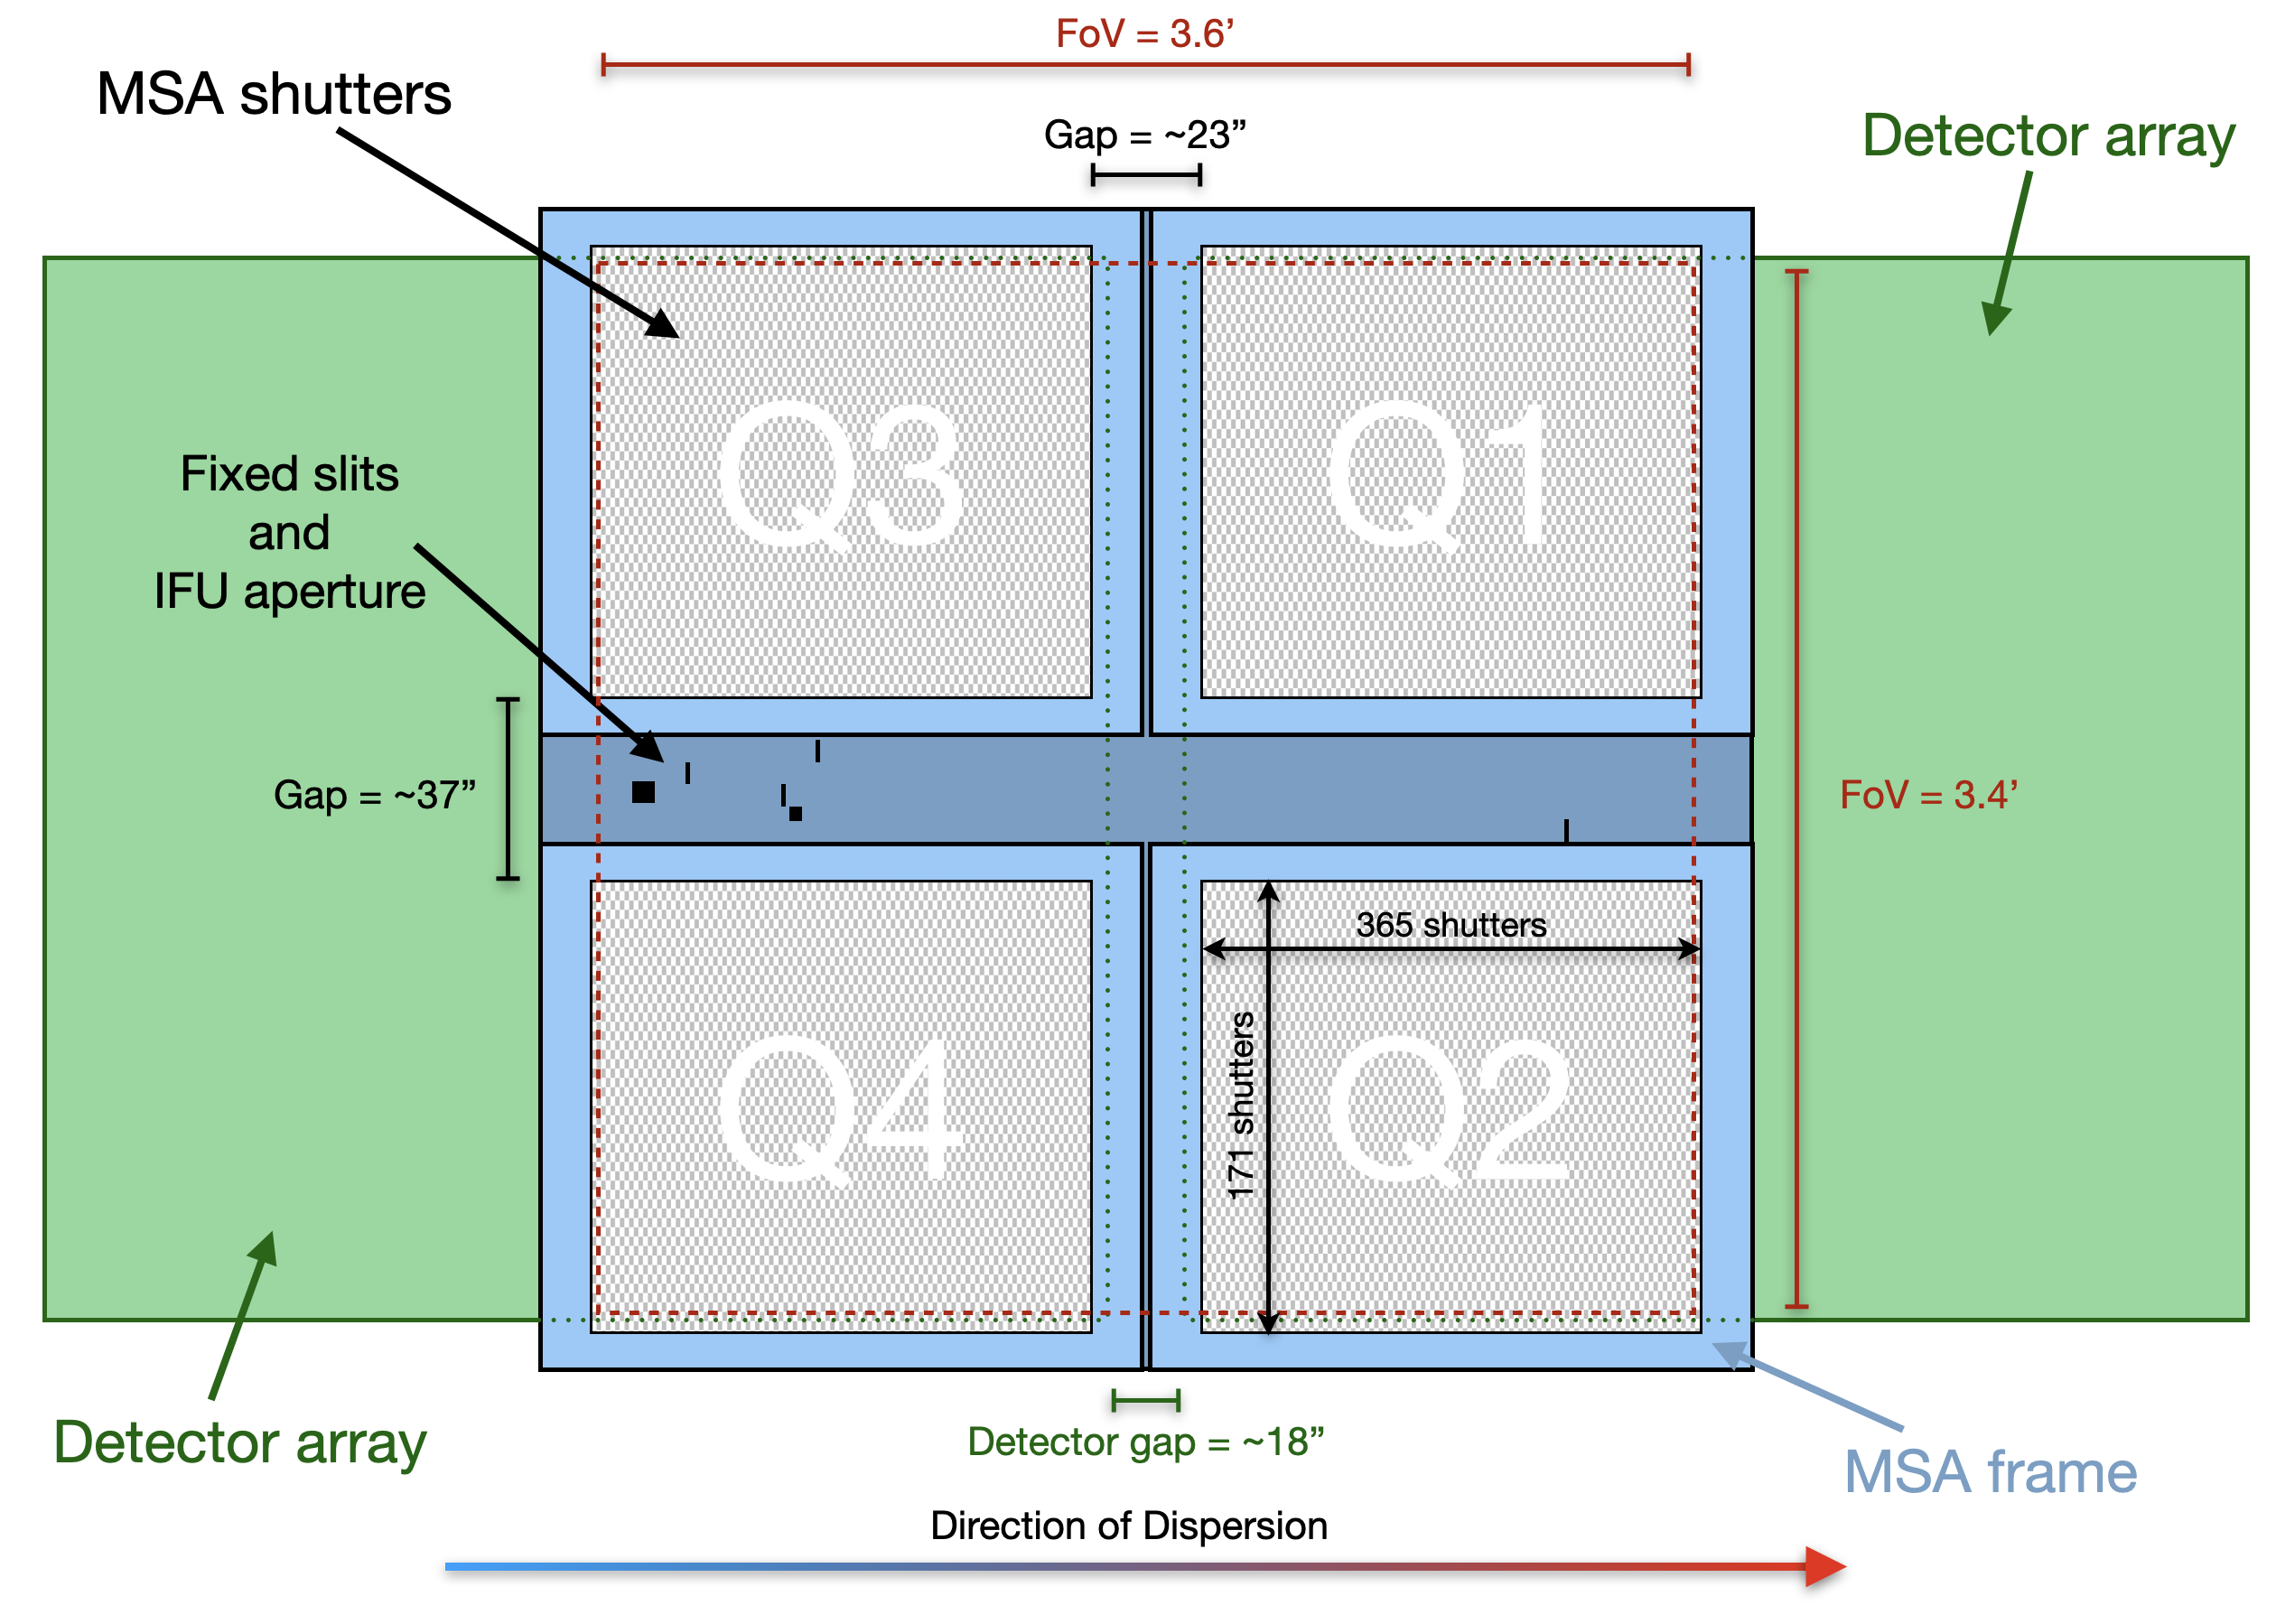
\includegraphics[scale=0.25]{assets/msa_ds_new.png}
  \label{fig:msa_shutter}
  \caption{Disposition de MSA dans le plan focal de NIRSpec. \customcite{Ferruit et al.}{2022A&A...661A..81F}}
\end{figure}

Parmi les instruments du \gls{jwst}, le \gls{nirspec} est un spectromètre sur la bande 0.6 - 5.3  µm, disposant de 3 modes de résolution : prism ($R \sim 100$), medium grating ($R \sim 1000$), high grating ($R \sim 2700$) \cite{nirspec}. L'un des atouts principaux de \gls{nirspec} est son \gls{msa}, une grille de près de 250 000 obturateurs, couvrant une surface de 3.6' x 3.4' sur le ciel, chacun pouvant être individuellement ouvert ou fermé \cite{msa} (voir \ref{fig:msa_shutter}). Ceci permet d'observer dans le mode \gls{mos} de \gls{nirspec}. Comme son nom l'indique, la spectroscopie multi-objet permet d'étudier le spectre de plusieurs objets dans un même champ, mais la grille d'obturateurs apporte également un outil fondamental dans l'extraction des spectres : la soustraction du fond.

\subsection{Fond, Nodding et Slitlet}

Lorsqu'on s'intéresse à des sources de faible brillance, le flux lumineux mesuré peut rapidement se trouver dominer par les émissions du fond. Que ce soit le fond diffus infrarouge, produit par des sources extragalactiques non résolues, la lumière zodiacale, produite par la poussière interplanétaire, le rayonnement de la Voie Lactée ou l'émission thermique du JWST lui-même, l'infrarouge est un domaine facilement parasité par des signaux indésirables \cite{jwst_background}. De plus, la nature de ses composantes fait de ce fond un signal anisotrope. Il n'est donc pas si simple d'en établir un modèle universel à soustraire de façon systématique. On a la mesure du fond en fonction de la longueur d'onde ci dessous \ref{fig:background_jwst} : 

\begin{figure}[H]
  \centering
  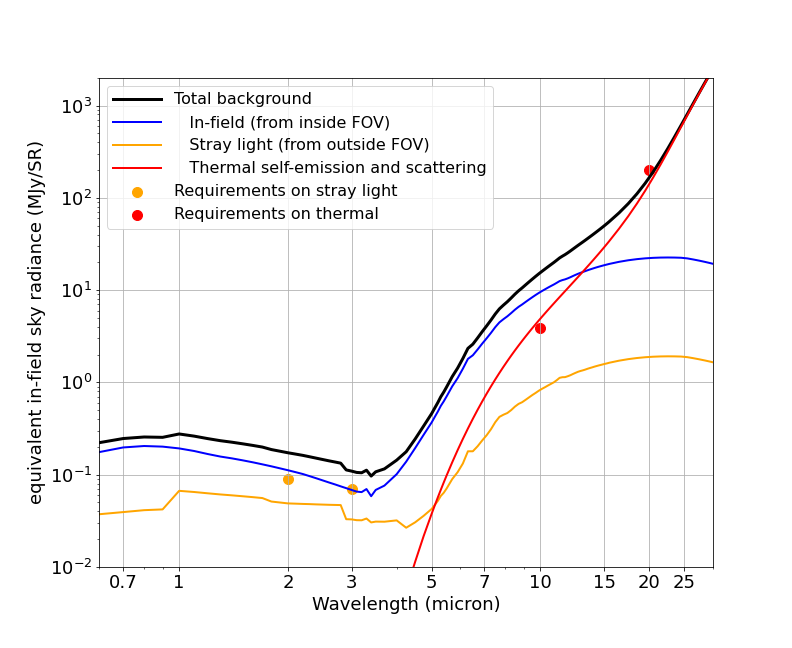
\includegraphics[scale=0.4]{assets/background_jwst.png}
  \label{fig:background_jwst}
  \caption{Flux par unité d'angle solide reçu par le JWST en fonction de la longueur d'onde. On remarque qu'à mesure que $\lambda$ augmente, l'émission thermique du télescope domine. \customcite{STScI}{jwst_background}}
\end{figure}


Cependant, il reste tout de même envisageable de corriger ce signal parasite. En effet, en ouvrant les obturateurs à proximité de celui imageant la source, il devient possible d'extraire le fond localement autour de la source, que l'on peut alors soustraire au spectre de cette dernière.

La configuration habituelle consiste en l'ouverture de 3 obturateurs dans la direction perpendiculaire à la direction de dispersion, on parlera par la suite de \textit{Slitlet}. On réalise alors 3 expositions, chacune en orientant le télescope de façon à avoir la source dans un obturateur différent : il s'agit du nodding. Ce mouvement entre chaque exposition offre également un autre avantage au travers du \textit{dithering}. La \gls{psf} de \gls{nirspec} est effectivement de $0.08 ''$ à $\lambda = 2.46 \mu m$ \cite{10_1051_0004_6361_202142663}. 
Comme $PSF \propto \lambda$, on a une \gls{psf} variant de $0.02 ''$ à $0.17''$ le long de la plage de longueur d'onde observable. Comme la taille d'un pixel est $\sim 0.1''$ dans la direction spatiale, la \gls{psf} est sous échantillonnée presque partout. Le dithering permet alors d'améliorer cet échantillonnage par des corrections sub-pixels, mais également de s'affranchir des éventuels pixels défectueux ou des rayons cosmiques.

On résume ceci dans la figure \ref{fig:msa_slitlet}.


\begin{figure}[H]
  \centering
  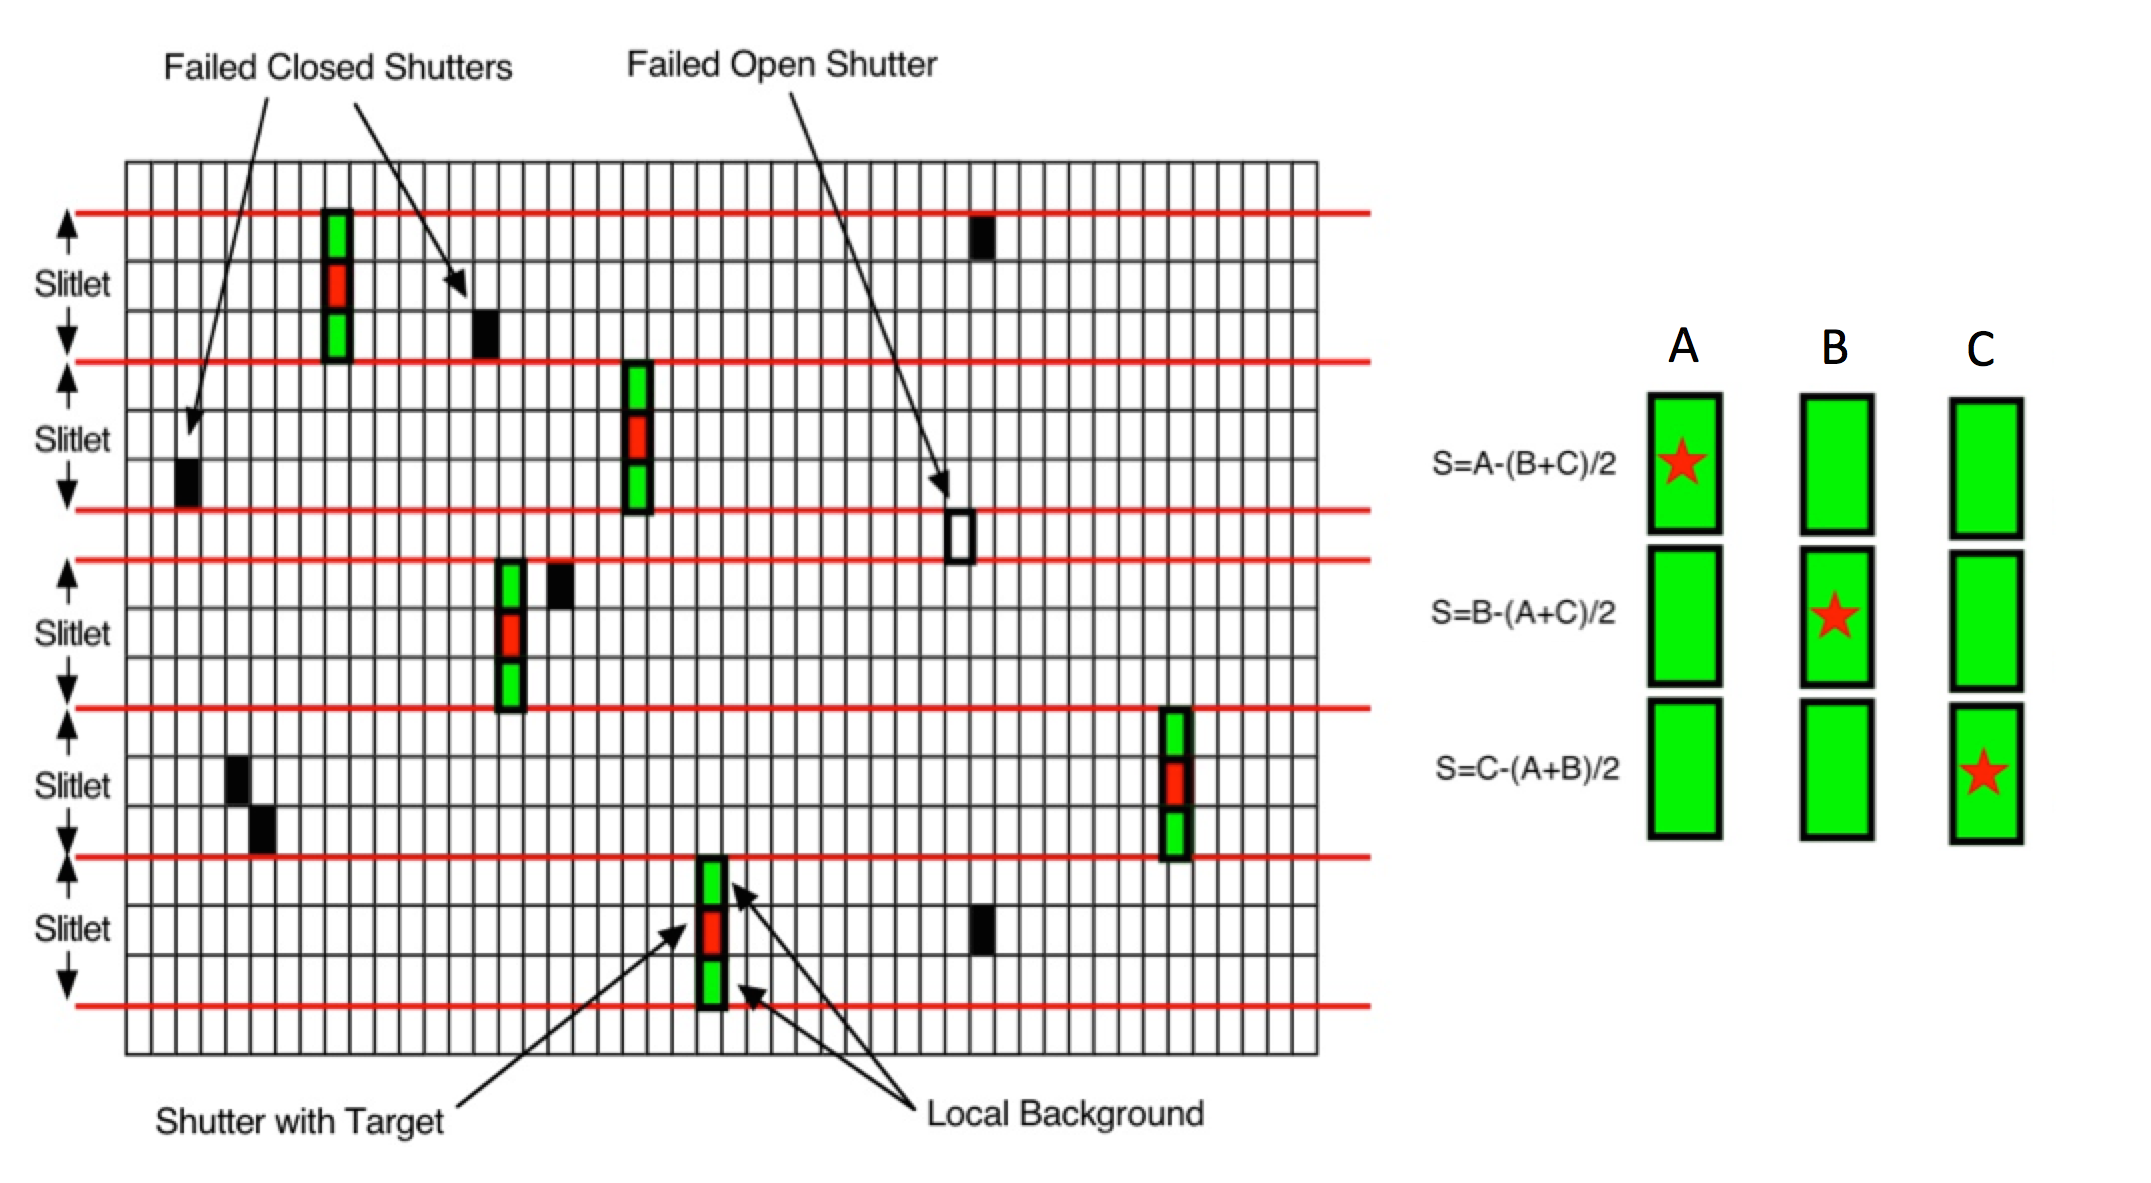
\includegraphics[scale=0.2]{assets/MSA_sky_strategy.png}
  \label{fig:msa_slitlet}
  \caption{Schéma de MSA et de slitlets. On réalise des séries de 3 images, chacune ayant la source dans un obturateur différent, et on utilise les 2 obturateurs restant pour déterminer le spectre du fond. \customcite{NIRSpec Instrument Development Team}{mos}}
\end{figure}

\subsection{Le pipeline JWST}

Le code permettant de traiter les données reçues du JWST, appelé pipeline (figure \ref{fig:jwst_pipeline}), se décompose en 3 grandes étapes, celles ci étant de plus en plus spécifique aux types de données que l'on cherche à étudier à mesure que l'on progresse dans le pipeline.

Ainsi, dans notre cas, les 3 étapes sont telles que :\\


\begin{minipage}{.5\linewidth}
  \begin{itemize}
    \item \textbf{Detector 1} : Applique les corrections au niveau du détecteur, tel que le masquage des pixels morts/chauds et des rayons cosmiques, la linéarisation du nombre d'\gls{adu}, la suppression du biais et du courant d'obscurité... Cette étape est la même pour tous les instruments du \gls{jwst}.
    \item \textbf{Spectroscopy 2} : Applique des modifications optiques, telles que la correction de champ plat et des pertes de lumières liées aux barres séparant les obturateurs, mais calibre également la photométrie et les données \gls{wcs}, associant à chaque pixel des coordonnées spatiales et spectrales. C'est ici que les images de chaque slitlets sont extraites de l'image initiale et que la soustraction du fond s'applique.
    \item \textbf{Spectroscopy 3} : Combine plusieurs expositions entre elles, appliquant ainsi le dithering / nodding discuté plus tôt, ré-échantillonne les images et extrait les spectres de celles-ci.
  \end{itemize}
  \end{minipage}
  \hfill
  \begin{minipage}{.5\linewidth}
  \centering
  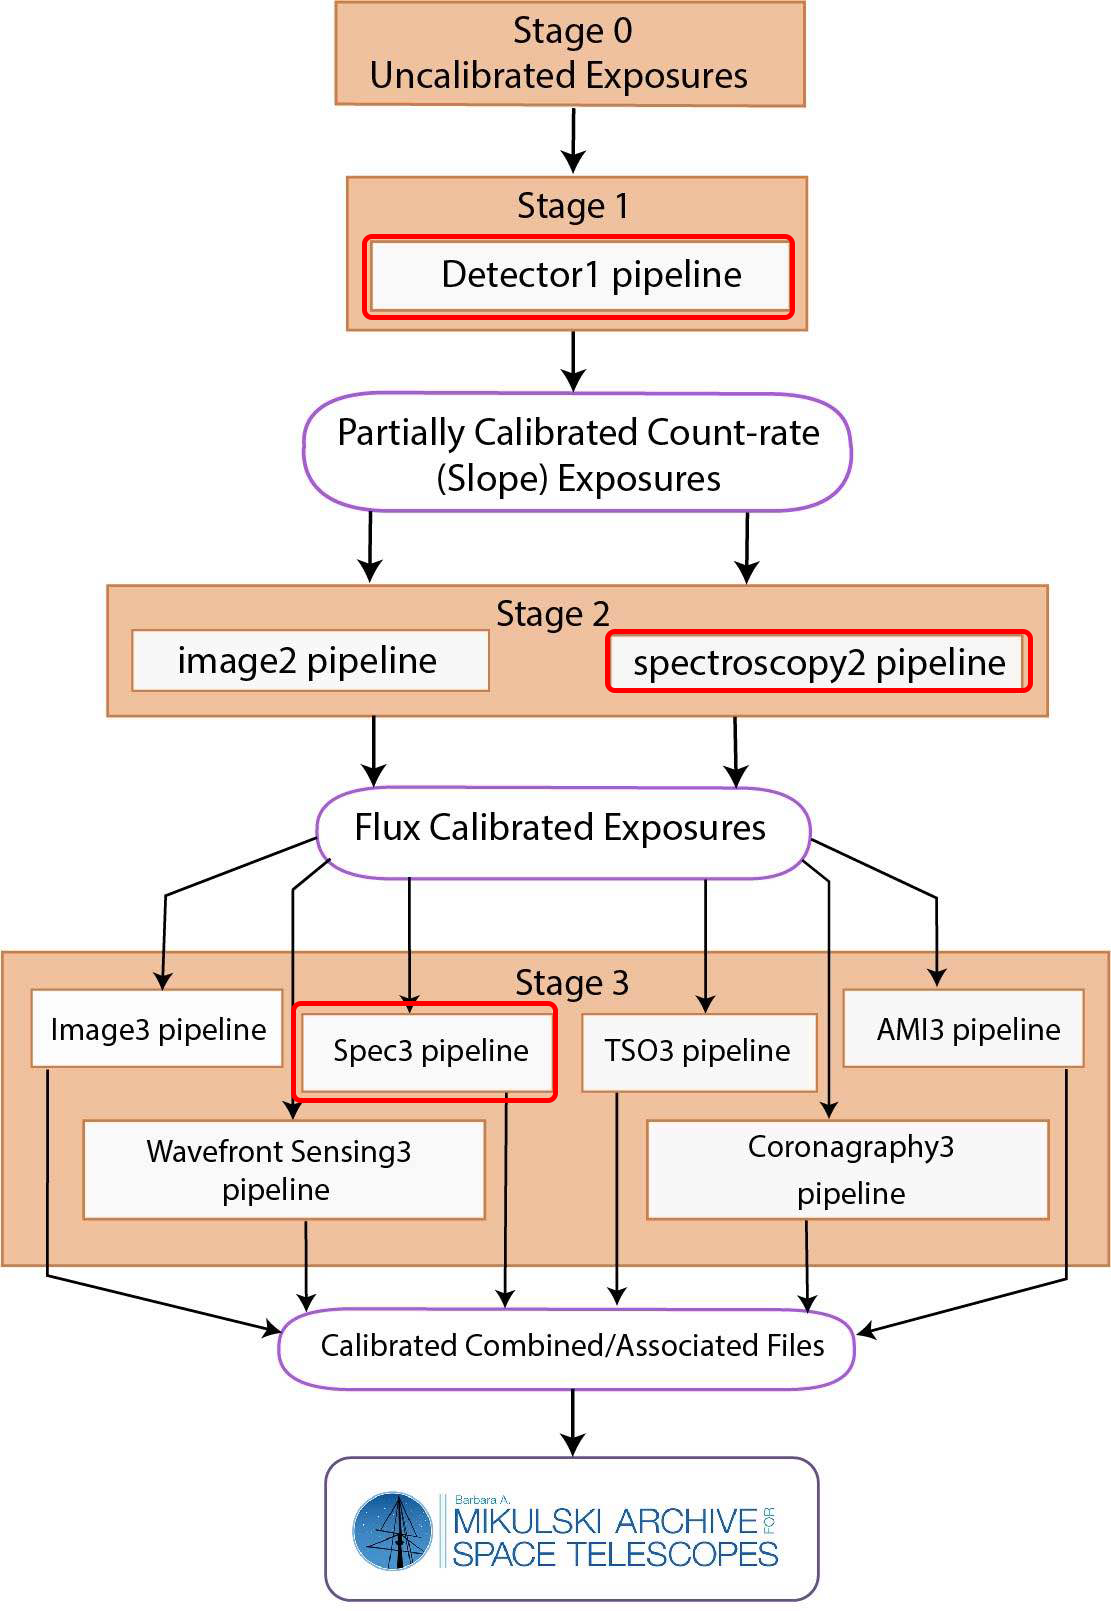
\includegraphics[scale=0.15]{assets/jwst_pipeline.jpg}
  \label{fig:jwst_pipeline}
  \captionof{figure}{Schéma des différentes étapes du pipeline. Les étapes adaptées à nos données sont encadrés en rouge. %TODO la citation}
  
  \end{minipage}








\printnoidxglossaries

\printbibliography %Prints bibliography


\end{document}
